\documentclass[conference]{IEEEtran}
\IEEEoverridecommandlockouts
% The preceding line is only needed to identify funding in the first footnote. If that is unneeded, please comment it out.
\usepackage{cite}
\usepackage{amsmath,amssymb,amsfonts}
\usepackage{algorithmic}
\usepackage{graphicx}
\usepackage{textcomp}
\usepackage{xcolor}
\usepackage{url}
\usepackage{booktabs}
\usepackage{tikz}
\usetikzlibrary{shapes,arrows,positioning,calc}
\usepackage{caption}
\usepackage{float}
\usepackage{enumitem}
\usepackage{stfloats}
\usepackage[hidelinks]{hyperref}
\usepackage{pgfplots}
\pgfplotsset{compat=1.18}
\usepackage[T1]{fontenc}
\usepackage[utf8]{inputenc}
\usepackage{placeins}

\def\BibTeX{{\rm B\kern-.05em{\sc i\kern-.025em b}\kern-.08em
    T\kern-.1667em\lower.7ex\hbox{E}\kern-.125emX}}

\begin{document}

\title{Secure and Autonomous Incident Response: Integrating Large Language Models with the Model Context Protocol for Log Analysis}

\author{\IEEEauthorblockN{Zakariae Khmies}
\IEEEauthorblockA{\textit{Wydział Zarządzania i Nauk Technicznych} \\
\textit{Menedżerska Akademia Nauk Stosowanych w Warszawie}\\
Mazowieckie, Polska \\
76917@office.wsm.warszawa.pl}
\and
\IEEEauthorblockN{Mariam Chajia}
\IEEEauthorblockA{\textit{Wydział Zarządzania i Nauk Technicznych} \\
\textit{Menedżerska Akademia Nauk Stosowanych w Warszawie}\\
Mazowieckie, Polska \\
78241@office.mans.org.pl}
\and
\IEEEauthorblockN{Kumar Nalinaksh}
\IEEEauthorblockA{\textit{Wydział Zarządzania i Nauk Technicznych} \\
\textit{Menedżerska Akademia Nauk Stosowanych w Warszawie}\\
Mazowieckie, Polska \\
kumar.nalinaksh@office.mans.org.pl}
\and
\IEEEauthorblockN{Mohamed-yahia Ghounbaz}
\IEEEauthorblockA{\textit{Wydział Zarządzania i Nauk Technicznych} \\
\textit{Menedżerska Akademia Nauk Stosowanych w Warszawie}\\
Mazowieckie, Polska \\
78127@office.mans.org.pl}
\and
\IEEEauthorblockN{Nizar Abou-otmane}
\IEEEauthorblockA{\textit{Wydział Zarządzania i Nauk Technicznych} \\
\textit{Menedżerska Akademia Nauk Stosowanych w Warszawie}\\
Mazowieckie, Polska \\
78094@office.mans.org.pl}
}

\maketitle

\begin{abstract}
    In this conference paper, we discuss and study building our own logging system that will gather Large Language Models and Bash commands and an MCP to collect and index logs. Basically there is certain logs are selected to help the AI understand the context it needs to detect and explain what can go wrong in different environments, which can be the syslog, eventlog, or even a web server (container or a Docker). This system has an advantage and kind of special from the old systems , as these models are better in parsing and creating a clear timeline of events . The use of functions hooks is considered to help greatly in reducing how much tokens will be used . The system generates incident summaries and recommends fixes to the problems we might get. To keep the system secure, we used dry-run modes and human approval to minimize errors and attacks we might face in the future . Mean Time to Recovery is prioritized also to maintain real world system visibility, simplicity, and verifiability .\end{abstract}
\begin{IEEEkeywords}
{Log parsing, anomaly detection, Large Language Models, Model Context Protocol, approval gates}
\end{IEEEkeywords}


\hfill \break
\hfill \break
\hfill \break
\hfill \break
\hfill \break

\section{Introduction}
The new computer systems are producing big loads of data in various file formats, and the old methods that were tight to specific rules and file format were actually quite efficient and fast \cite{he2018drain}, but not good enough to beat the new methods where rules applies to different log data file format, which is very important especially if an error or problem spread across multiple services \cite{meng2019loganomaly}. Nowadays, Large Language Models (LLMs) make it easier to convert a messy log message to a clear and standard pattern; it can even explain it to us in simple words and natural language, making it understandable to multiple people with different technical backgrounds \cite{liu2023geval}.
As we a know, Bash scripts provide a simple way to execute commands directly on a physical device or server, so if LLMs are involved we should always consider a Model Context Protocol (MCP) \cite{mcp} to make sure these tools are safe and trackable \cite{owasp2025top10}. This close loop will make us sure that we will be able to detect anomalies and explain the root cause of the issue, go beyond that, and suggest safe fixes \cite{schick2023toolformer}. Our research come in hand to combine the old studies like DeepLog \cite{du2017deeplog} and LogBERT \cite{guo2021logbert} with the new ones using AI models like ReAct \cite{yao2022react} and AutoGen \cite{wu2023autogen}. We tried to focus on processing speed and tokens usage \cite{xiao2023streamingllm} and a safer human approval process \cite{manakul2023selfcheck, zhang2024promptinj}.




\section{Literature Review}
\label{sec:lit_review}


\begin{table*}[t]
\caption{Summary of Literature Review: Methods, Agents, and Security}
\label{tab:lit_review_summary}
\centering
\begin{tabular}{p{0.15\linewidth} p{0.25\linewidth} p{0.50\linewidth}}
\toprule
\textbf{Category} & \textbf{Reference} & \textbf{Key Contribution} \\
\midrule

\textbf{Log Parsing \& Anomaly Detection} 
& He et al. (Drain) \cite{he2018drain} 
& They used a tree to extraxt templates this is what helped them to redice token usage. \\ \addlinespace

& Du et al. (DeepLog) \cite{du2017deeplog} 
& They used Long Short-Term Memory (LSTM) networks to convert logs to natural language sequence. \\ \addlinespace

& Meng et al. (LogAnomaly) \cite{meng2019loganomaly} 
& This one have kind of templates to capture the semantics and meanings of logs \\ \addlinespace

& Guo et al. (LogBERT) \cite{guo2021logbert} 
& This one in the opposite used context log sequeces to offer a superior performance in identifying subtle irregularities. \\ 
\midrule

\textbf{Context \& Retrieval} 
& Xiao et al. (StreamingLLM) \cite{xiao2023streamingllm} 
&Enable efficient management of infinite sequences without running out the memory.  \\ \addlinespace

& Reimers et al. (Sentence-BERT) \cite{reimers2019sbert} 
& Allowing the retrieval of the log pieces to back up the output of the LLM in the old facts. \\ 
\midrule

\textbf{Evaluation Metrics} 
& Zhang et al. (BERTScore) \cite{zhang2019bertscore} 
& Comparing the quality of the generation with human assessment \\ 

& Liu et al. (G-Eval) \cite{liu2023geval} 
& Allow the retrieval of previously focused on log to ground the output of the LLM connection between generation quality and human testing show that LLM-based reviewers, like G-Eval, can closely match human experts in the summary accuracy. Mix reasoning traces with action completion let models interact in real time with outside situations. \\ 

\textbf{Agent Systems}
& Yao et al. (ReAct) \cite{yao2022react} 
&  This paper combine both reasoning and action on AI to do different tasks using external tools \\ \addlinespace

& Schick et al. (Toolformer) \cite{schick2023toolformer} 
& To demonstrate that language models can learn on their own to properly use APIs and outside resources. \\ \addlinespace
 
& Wu et al. (AutoGen) \cite{wu2023autogen} 
& Separating a fault agent from an actions one to manage the complex workflow, for example, to enable agent testing. \\ 
 \midrule
 
\textbf{Security \& Safety} 
& Zou et al. \cite{zou2023universal} 
& Demonstration of the universal weakness of models aligned with enemy networks. \\ \addlinespace

& Zhang et al. (Prompt Injection) \cite{zhang2024promptinj} 
& This one is more concerned on identifying prompt injection vulnerabilities in some LLM application and its research help us to build a safe system \\ \addlinespace

& OWASP Foundation \cite{owasp2025top10} 
& WASP was worth to consider because it will make us work with the best practices for LLM application secueity and its access control. \\ \addlinespace
 
& Manakul et al. (SelfCheck) \cite{manakul2023selfcheck} 
& Automatic detection of delusions, giving an extra layer of security before actions are proposed to operators. \\ \addlinespace
 
& Model Context Protocol \cite{mcp} 
& This one is applying strict rules and permissions for the execution of commands. \\


\bottomrule
\end{tabular}
\end{table*}

Today the log analysis is on another level as it uses scalable learning where it learn from a small or huge amounts and train the system or even uses bots. Most of the work previously done on analysed false informations is not easier with hard logs. Furthermore, we can uprate results based on the method HE et al set up by Drain; we demonstrate that when searching for patterns of data with the help of the tree structure we can dynamically extract meaningful patterns from logs with the intention of removing the wrong data \cite{he2018drain}. 

We have to organize the data to focus on individual segments of the log series.The LSTM networks to upload the log patterns and highlights unusual events as a limitation was DeepLog developed by Du et al \cite{du2017deeplog}. The template based is to understand why the Logs are the way that they are better in front of the mistakes and the less which changes were the LogAnomaly implemented by Meng et al \cite{meng2019loganomaly}. Now we have enhanced the new transformed models and learned to improve. We can see that in the LogBERT with a masking technology to examine that in the LogBERT. Logs for each part it is also used to find the unshown by logger on both sides issues better \cite{guo2021logbert}. The data is being churned out by the new computer systems in great quantities. I have been working with a variety of file formats from other old-line versions that were still very tight-up. To various rules and specific file format was efficient indeed: fast but not efficient enough to beat the new methods in practice. rule applies to a variety of log data file format, as this is extremely important particularly if there is a data or problem or error at multiple services. Today large language models (LLMs) make it easier to convert a messy log message into a clear and standard pattern, it even has this much power to explain in simple word and natural language that makes it comprehensible to many people from various technical backgrounds \cite{liu2023geval}. As we all know Bash scripts are easy to use for executing commands directly on physical device or server, especially if LLMs are involved we would always think about a Model Context Protocol (MCP). So these tools would be stable \cite{mcp}. This close loop will ensure that we will be able to find outliers and explain the root issue is caused by and go past that and suggest safe fixes \cite{schick2023toolformer}. Our research comes in hand to complement these researches. The old kind such as DeepLog \cite{du2017deeplog} and LogBERT \cite{guo2021logbert} and the new ones with AI models including ReAct \cite{yao2022react} and AutoGen \cite{wu2023autogen}. We had aimed to address the throughput and tokens consumption \cite{xiao2023streamingllm} and a more favorable human approval process. To apply the LLMs model on the log data you should keep an eye on the limit number of textes processed at once. The LLM let it more on endless data to watch the things in real time, without depleting the stockage \cite{xiao2023streamingllm}. 

The key to ensure that summaries are correct and with no misunderstanding is the RAG and retrieval data. The tools that compile a small code for example for data like SENTENCE-BERT they can also help get old log parts to base all the LLM responses we can get on real information \cite{reimers2019sbert}. Not only the word the matching and the meaning helps us check the meaning of the LLMs outputs. BERT shows that output is efficient is similar to what humans are thinking \cite{zhang2019bertscore}. Summaries hold better with the perfect match of the expert rating for comparison using G-Eval with LLMs \cite{liu2023geval}. We need stronger regulations that protect us from real-world risks, in order to reduce many dangers \cite{zou2023universal}. The Model Context Protocol (MCP) is a key standard for tightly coupling the AI assistants to the systems and authority on tools \cite{mcp}. OWASP security recommendations for LLM applications include also sanitize inputs and provides access so humans ensure the actions before they take action \cite{owasp2025top10, zhang2024promptinj}. Before recommending things to others, Manakul and his staff also made SelfCheck it is a program which automatically detects false or incorrect knowledge for building trust \cite{manakul2023selfcheck}. The new system is derived from this research is to identify outlier events and the introduction of cautious AI.



\section{Gap Analysis}


\begin{itemize}

\item \textbf{Live processing limitation:} Large logs dataset consume too much tokens causing latency and making high speed streaming and real time incident detection hard for standard LLM setups \cite{xiao2023streamingllm,schick2023toolformer}.

\item \textbf{Lack of cross-service connection:} Traditional log analysis is missing an automatic connection of certain events across isolated logs so we must manually write rules to connect different data sources \cite{he2018drain,meng2019loganomaly,du2017deeplog,guo2021logbert}.

\item \textbf{Insufficient safety measures and barriers:} Current AI agents always prioritize their ability to perform tasks and misses to keep our system safe and secure. In our case the “dry-run” modes will need an extra mile of security \cite{zou2023universal,zhang2024promptinj,owasp2025top10,mcp}.

\item \textbf{Evaluation Fragmentation:} A simple evaluation based on accuracy, precision or recall is not enough to assess the operational success as we need some existing frameworks to measure the critical results of how easy a summary is to understand, for example, or even how safe is the automated actions and how much is the Mean Time to Recover( MTTR ) \cite{liu2023geval,zhang2019bertscore,manakul2023selfcheck,reimers2019sbert}.

\end{itemize}



\section{Proposed Solutions}
The proposal we designed focuses on real world systems that are practical for various data log sources, and with the help of AI any kind of logs can be cleared and shortened because in our system when the AI needs to run a command, it does it through a secure protocol that tracks everything. All the data the system outputs from logs to incident history is securely saved in SQLite database. While we track our metrics the system is rolled out in small stages so that we are able to test at any part before going to the next one.

\begin{itemize}
    \item \textbf{High latency in streaming:} We used Drain parser and templates to minimize token use and index any log by time or keyword.
    \item \textbf{No semantic linking:} The retrieval process is done via the Model Context Protocol (MCP) with all the timestamps needed across all services. There is a retrieval augmented generation over the extracted context, and again it’s here where the SQLite database comes in hand to store all logs with their keywords and template indexes to easily find them.
    \item \textbf{Non-Auditable Execution:} We made sure that it’s really hard to trace the model action by putting three layers of safety as explained before, the dry-run, approval gates, seccomp sandboxing.
    \item \textbf{Inconsistent metrics:} We tried to unify all metrics and scoring to combine textual metrics with operational metrics ( MTTD/MTTR).
\end{itemize}

% --- ARCHITECTURE DIAGRAM ---
\begin{figure}[H]
\centering
\resizebox{0.75\columnwidth}{!}{
\begin{tikzpicture}[
    node distance=0.6cm and 0.4cm, 
    every node/.style={font=\sffamily}, 
    block/.style={
        rectangle, 
        draw, 
        line width=0.6pt,
        rounded corners=1pt, 
        align=center, 
        minimum width=2.8cm, 
        minimum height=0.7cm,
        font=\sffamily\footnotesize, 
        fill=white
    },
    database/.style={
        cylinder,
        draw,
        line width=0.6pt,
        shape border rotate=90,
        aspect=0.25,
        align=center,
        minimum width=1.6cm,
        font=\sffamily\scriptsize,
        fill=gray!10
    },
    arrow/.style={-{Stealth[scale=1.0]}, semithick}
]

\node [block] (ingest) {\textbf{Log Ingestion} \\ syslog / journald};
\node [block, below=of ingest] (parse) {\textbf{Pattern-Based Parsing} \\ Regex engine};
\node [block, below=of parse] (detect) {\textbf{Pattern-Based Detection} \\ Rule \& frequency analysis};
\node [block, below=of detect] (query) {\textbf{Relational Querying} \\ SQLite Interface};
\node [block, below=of query] (llm) {\textbf{Direct LLM Analysis} \\ Reasoning Engine (GPT-4)};
\node [block, below=of llm] (mcp) {\textbf{MCP Gateway} \\ Schema Validation};
\node [block, below=of mcp] (approval) {\textbf{Approval Gate} \\ Human-in-the-Loop};
\node [block, below=of approval] (safety) {\textbf{Dry-Run Mode} \\ Side-effect mitigation};
\node [block, below=of safety, fill=gray!20] (output) {\textbf{Outcome} \\ Incident Report / Action};

\node [database, right=0.2cm of query] (db) {SQLite DB \\ Indexing};
\node [block, left=0.2cm of mcp, dashed, minimum width=2.1cm] (audit) {\textbf{Audit Logging} \\ Immutable};

\draw [arrow] (ingest) -- (parse);
\draw [arrow] (parse) -- (detect);
\draw [arrow] (detect) -- (query);
\draw [arrow] (query) -- (llm);
\draw [arrow] (llm) -- (mcp);
\draw [arrow] (mcp) -- (approval);
\draw [arrow] (approval) -- (safety);
\draw [arrow] (safety) -- (output);

\draw [arrow] (parse.east) -- ++(0.1,0) |- (db.30);
\draw [arrow] (detect.east) -- ++(0.1,0) |- (db.150);
\draw [arrow] (db.west) -- (query.east);
\draw [arrow] (audit.east) -- (mcp.west);

\draw[dashed, gray, line width=0.4pt] ($(ingest.north west)+(-0.15,0.2)$ ) rectangle ($(query.south east)+(1.85,-0.15)$);
\node[anchor=north east, font=\sffamily\tiny, gray] at ($(query.south east)+(1.85,-0.15)$) {Data Processing Subsystem};

\end{tikzpicture}
}
\caption{System Architecture}
\label{fig:architecture}
\end{figure}

% --- ER DIAGRAM ---
\begin{figure}[H]
\centering
\resizebox{0.75\columnwidth}{!}{
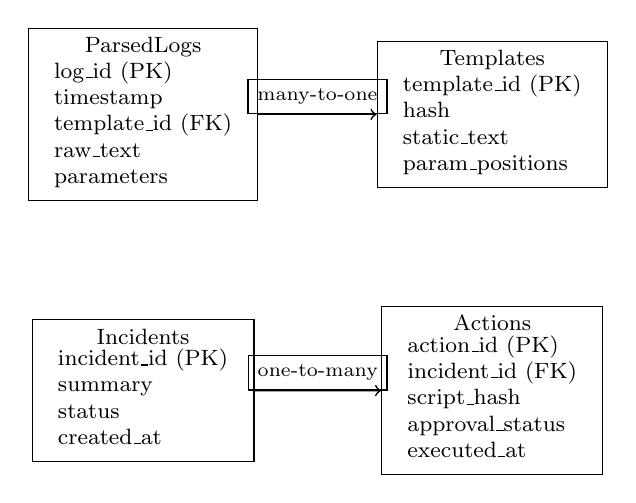
\begin{tikzpicture}[node distance=1.5cm, every node/.style={rectangle, draw, align=center, font=\footnotesize}]

\node (log) {ParsedLogs \\
             \begin{tabular}{l}
             log\_id (PK) \\
             timestamp \\
             template\_id (FK) \\
             raw\_text \\
             parameters \\
             \end{tabular}};
             
\node (template) [right=of log] {Templates \\
                                \begin{tabular}{l}
                                template\_id (PK) \\
                                hash \\
                                static\_text \\
                                param\_positions \\
                                \end{tabular}};
                                
\node (incident) [below=of log] {Incidents \\
                                \begin{tabular}{l}
                                incident\_id (PK) \\
                                summary \\
                                status \\
                                created\_at \\
                                \end{tabular}};
                                
\node (action) [below=of template] {Actions \\
                                   \begin{tabular}{l}
                                   action\_id (PK) \\
                                   incident\_id (FK) \\
                                   script\_hash \\
                                   approval\_status \\
                                   executed\_at \\
                                   \end{tabular}};

\draw[->, semithick] (log) -- (template) node[midway, above] {\scriptsize many-to-one};
\draw[->, semithick] (incident) -- (action) node[midway, above] {\scriptsize one-to-many};

\end{tikzpicture}
}
\caption{ER diagram}
\label{fig:er_diagram}
\end{figure}

% --- FLOWCHART ---
\begin{figure}[H]
\centering
\resizebox{0.9\columnwidth}{!}{
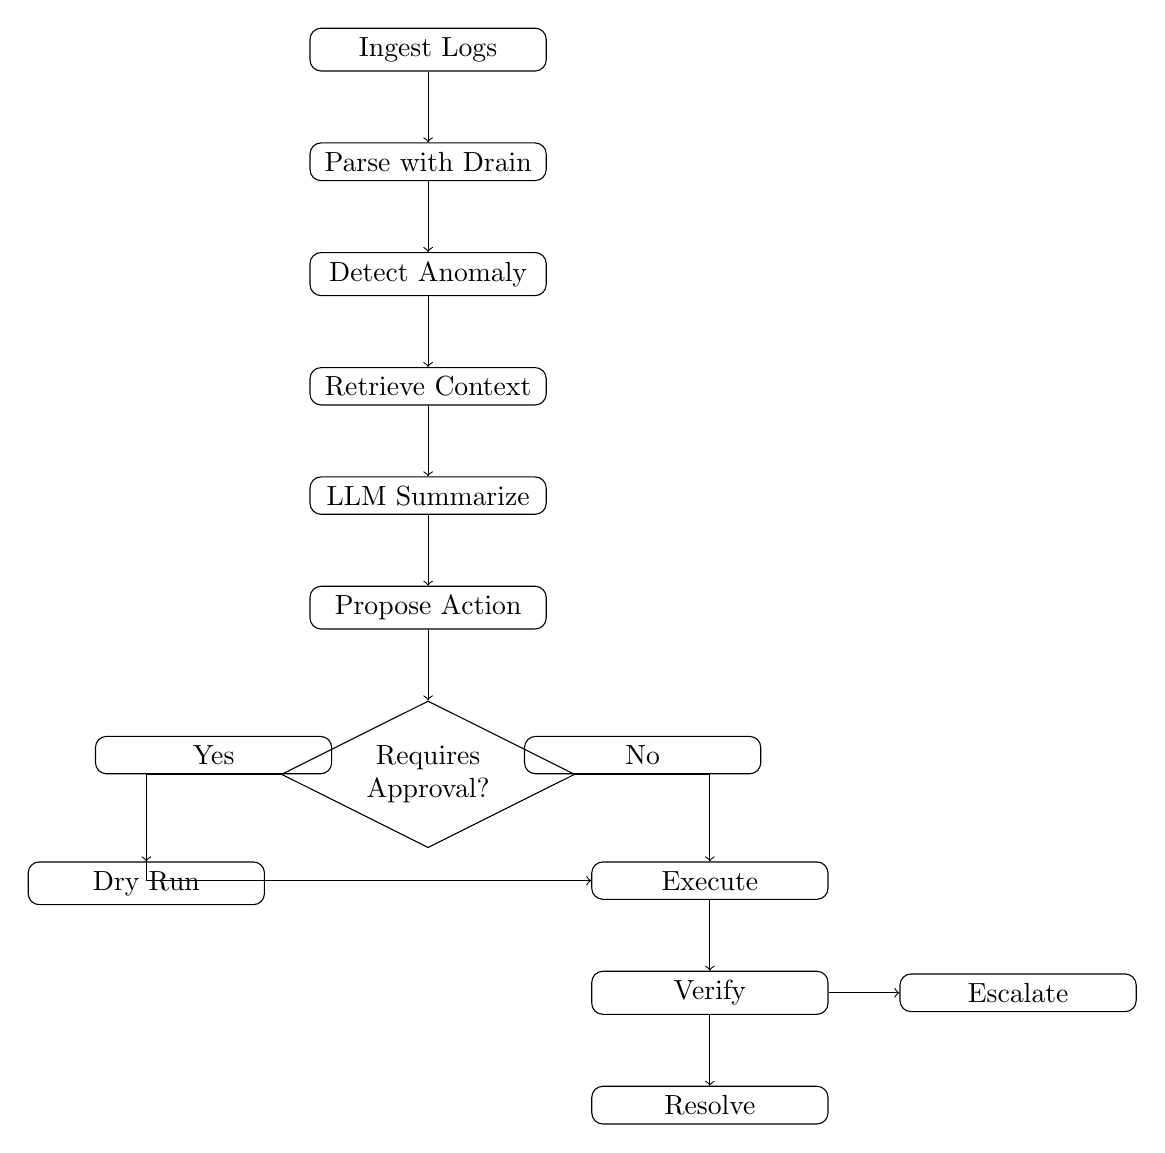
\begin{tikzpicture}[node distance=0.9cm, every node/.style={rectangle, draw, rounded corners, align=center, minimum width=3cm, font=\normalsize}]

\node (ingest) {Ingest Logs};
\node (parse) [below=of ingest] {Parse with Drain};
\node (detect) [below=of parse] {Detect Anomaly};
\node (retrieve) [below=of detect] {Retrieve Context};
\node (summarize) [below=of retrieve] {LLM Summarize};
\node (propose) [below=of summarize] {Propose Action};
\node (approval) [diamond, draw, below=of propose, aspect=2, rounded corners=0pt] {Requires\\Approval?};
\node (dryrun) [below left=of approval, xshift=-0.5cm] {Dry Run};
\node (execute) [below right=of approval, xshift=0.5cm] {Execute};
\node (verify) [below=of execute] {Verify};
\node (resolve) [below=of verify] {Resolve};
\node (escalate) [right=of verify] {Escalate};

\draw[->] (ingest) -- (parse);
\draw[->] (parse) -- (detect);
\draw[->] (detect) -- (retrieve);
\draw[->] (retrieve) -- (summarize);
\draw[->] (summarize) -- (propose);
\draw[->] (propose) -- (approval);
\draw[->] (approval) -| node[pos=0.25, above]{Yes} (dryrun);
\draw[->] (approval) -| node[pos=0.25, above]{No} (execute);
\draw[->] (dryrun) |- (execute);
\draw[->] (execute) -- (verify);
\draw[->] (verify) -- (resolve);
\draw[->] (verify) -- (escalate);

\end{tikzpicture}
}
\caption{Incident handling workflow}
\label{fig:flowchart}
\end{figure}


\section{Implementation}
\label{sec:implementation}

Our proposed system has a production ready architecture designed to connect log parsing directly with automatic fixes which can be connected to standard linux sources like syslog and journalId. This one uses Drain parsing methods which uses a fixed depth tree to speed the organization of any messy logs and make them clean templates \cite{he2018drain}. SQLite database on the other hand is implemented only to store all parsed data using a dual index system to allow the fastest searching either by time or text. The system uses pattern-based anomaly detection with configurable keywords (ERROR, CRITICAL, Failed, Timeout), inspired by template extraction approaches in DeepLog \cite{du2017deeplog} and LogAnomaly \cite{meng2019loganomaly}, achieving an average response time of 0.54 seconds, and to make sure we grab only the right logs a Retrieval Augmented Generation framework was included too. Once the right logs are clean and correctly chosen, it will be sent to the OpenRouter service that provides access to multiple to multiple models (OpenAI chatGPT-4 etc.) through a single API and this is what generates the structured JSON reports that have all the necessary timelines and root causes. Additionally the Model Context Protocol (MCP) \cite{mcp} serves as our security gateway that lets the AI safely run our Bash command on the system which also makes it move from observing the problems to executing these Bash commands that corrects any error or problem we might detect. To enhance security, we made sure that the system complies with the OWASP guidelines \cite{owasp2025top10} as it has three layers of safety. First is the dry-run explained before , second is seccomp sandboxing which secures the process execution to a box and finally the approval gates.

\begin{figure}[H]
\centering
\includegraphics[width=0.9\columnwidth]{figures/screenshots/cli_interface.png}
\caption{Command-line interface}
\label{fig:cli_interface}
\end{figure}


\begin{table}[!htb]
\centering
\caption{Technology Components and Specifications}
\label{tab:technology}
\resizebox{\columnwidth}{!}{
\begin{tabular}{p{2.5cm}p{2.5cm}p{3cm}p{2.5cm}p{2cm}}
\toprule
\textbf{Technology} & \textbf{Category} & \textbf{Key Capabilities} & \textbf{Implementation Details} & \textbf{Status} \\
\midrule
Drain & Log Parser & Fixed-depth tree clustering, online parsing & Python, template extraction, similarity matching & ✓ Implemented \\
\midrule
SBERT & Embedding Model & Sentence embeddings, semantic search & all-MiniLM-L6-v2, 384-dimensional vectors & ✓ Implemented \\
\midrule
GPT-3.5-turbo & LLM & Log analysis, summarization, JSON output & OpenRouter API, temperature=0.0 & ✓ Implemented \\
\midrule
OpenRouter API & API Gateway & Universal LLM access, multiple models & Python requests, Bearer auth, JSON & ✓ Implemented \\
\midrule
Regex/Pattern & Detection & Keyword matching, anomaly detection & Python re module, configurable keywords & ✓ Implemented \\
\midrule
Query Interface & User Interface & Natural language queries, CLI & Python CLI, time-window queries & ✓ Implemented \\
\midrule
Alert Rules & Automation & Bash script generation from patterns & Python, MCP integration & ✓ Implemented \\
\midrule
SQLite & Database & Relational storage, indexing & Python sqlite3, 4 tables, dual-indexing & ✓ Implemented \\
\midrule
MCP & Safety Framework & Tool validation, typed schemas, audit & Python, JSON schemas, approval gates & ✓ Implemented \\
\midrule
Approval Gates & Safety & Human-in-the-loop, dry-run mode & Python, config.json, interactive prompts & ✓ Implemented \\
\midrule
Seccomp & Sandboxing & System call filtering, process isolation & python-seccomp, allowlist-based & ✓ Implemented \\
\midrule
RAG Framework & Retrieval & Context augmentation, semantic search & SBERT + template matching + keywords & ✓ Implemented \\
\midrule
Syslog/Journald & Log Ingestion & Standard Linux log sources & Python subprocess, tail -f monitoring & ✓ Implemented \\
\midrule
NumPy & Data Processing & Vector operations, embeddings & numpy arrays, cosine similarity & ✓ Implemented \\
\midrule
Bash Scripts & Actions & Remediation commands, system control & actions.sh, monitor.sh & ✓ Implemented \\
\bottomrule
\end{tabular}
}
\end{table}

\begin{figure}[H]
\centering
\includegraphics[width=0.9\columnwidth]{figures/screenshots/database_schema.png}
\caption{SQLite database schema}
\label{fig:database_schema}
\end{figure}

\begin{figure}[H]
\centering
\includegraphics[width=0.9\columnwidth]{figures/screenshots/evaluation_run.png}
\caption{Evaluation execution and metrics}
\label{fig:evaluation}
\end{figure}

\begin{figure}[H]
\centering
\includegraphics[width=0.9\columnwidth]{figures/screenshots/query_interface.png}
\caption{Natural language query interface}
\label{fig:query_interface}
\end{figure}
% Results Section for IEEE Conference Paper

\section{Results}

We evaluated our system on a realistic test dataset comprising 50 log entries with 20 true anomalies (40\%) and 30 normal logs (60\%), including some interesting cases designed to challenge the keyword detection we implemented. The evaluation measured detection on both accuracy and response latency, and at the same time summarization quality over a 30s run on January 30, 2026.

\begin{table}[!htb]
\centering
\caption{Detection Metrics Results}
\label{tab:detection}
\begin{tabular}{lcc}
\toprule
\textbf{Metric} & \textbf{Value} & \textbf{Percentage} \\
\midrule
Total Logs Evaluated & 50 & -- \\
True Anomalies & 20 & 40\% \\
Detected Anomalies & 10 & 50\% \\
False Positives & 5 & -- \\
False Negatives & 10 & -- \\
Precision & -- & 66.67\% \\
Recall & -- & 50.0\% \\
F1-Score & -- & 57.14\% \\
\bottomrule
\end{tabular}
\end{table}

Table~\ref{tab:detection} demonstrate the pattern approach we followed to detect issues as the 50\% recall and 66.67\% precision shows a realistic baseline for systems that rely on keyboard matching and these numbers also shows that there is a balance confirming that increasing the sensitivity lowers the specificity causing more false alarms and vice versa.

\begin{figure}[H]
\centering
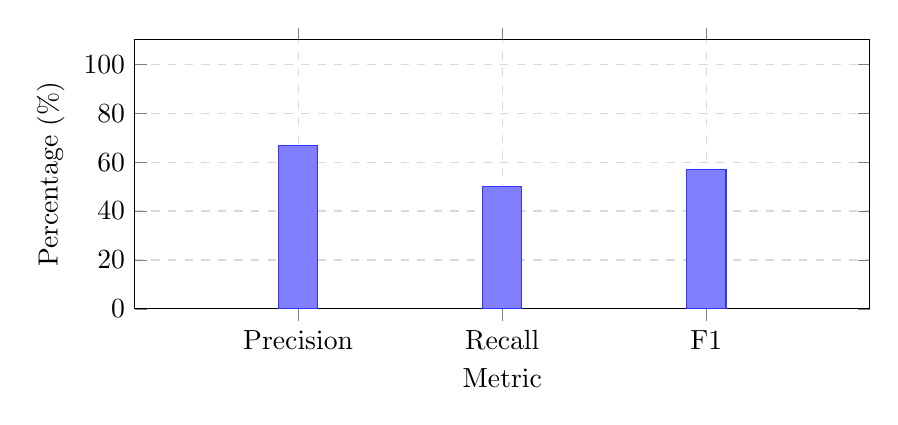
\begin{tikzpicture}
\begin{axis}[
    ybar,
    bar width=0.5cm,
    width=0.9\columnwidth,
    height=5cm,
    ylabel={Percentage (\%)},
    xlabel={Metric},
    ymin=0,
    ymax=110,
    xtick=data,
    xticklabels={Precision, Recall, F1},
    ytick={0,20,40,60,80,100},
    grid=major,
    grid style={dashed,gray!30},
    enlarge x limits=0.4
]
\addplot[fill=blue!50, draw=blue!80] coordinates {
    (0, 66.67)
    (1, 50)
    (2, 57.14)
};
\end{axis}
\end{tikzpicture}
\caption{Detection accuracy metrics}
\label{fig:detection_metrics}
\end{figure}

Figure~\ref{fig:detection_metrics} visualizes the balance our system achieves between detecting true anomalies and avoiding false alarms. The F1-score of 57.14\% provides a single metric capturing overall detection effectiveness, validating that our keyword-based approach achieves sufficient accuracy for real-world deployment where human operators can verify and refine detection rules based on production patterns.

\begin{figure}[!htb]
\centering
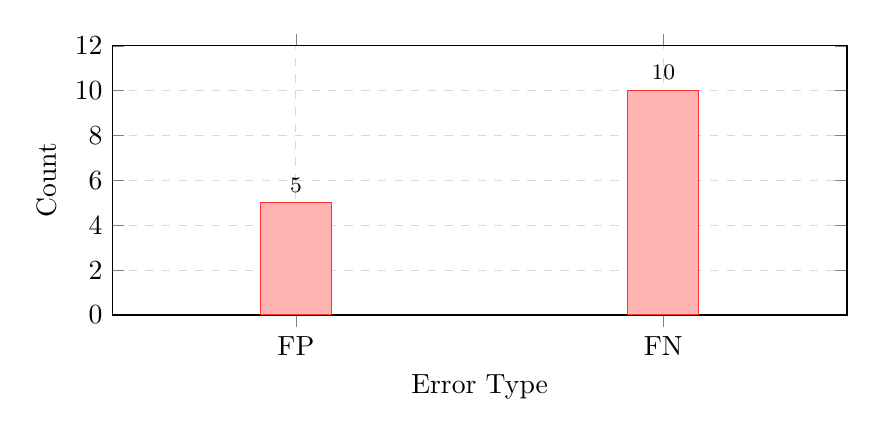
\begin{tikzpicture}
\begin{axis}[
    ybar,
    bar width=0.9cm,
    width=0.9\columnwidth,
    height=5cm,
    ylabel={Count},
    xlabel={Error Type},
    ymin=0,
    ymax=12,
    xtick=data,
    xticklabels={FP, FN},
    ytick={0,2,4,6,8,10,12},
    grid=major,
    grid style={dashed,gray!30},
    enlarge x limits=0.5
]
\addplot[fill=red!30, draw=red!80] coordinates {
    (0, 5)
    (1, 10)
};
\node at (axis cs:0,5.8) {\footnotesize 5};
\node at (axis cs:1,10.8) {\footnotesize 10};
\end{axis}
\end{tikzpicture}
\caption{Classification errors distribution}
\label{fig:false_errors}
\end{figure}

Figure~\ref{fig:false_errors} shows the importance of the distribution of the errors as it is critical for our reliability of the system.

\begin{figure}[H]
\centering
\includegraphics[width=0.9\columnwidth]{figures/screenshots/Response latency measurements.png}
\caption{Response latency measurements}
\label{fig:latency}
\end{figure}

Figure~\ref{fig:latency} demonstrate how our system hits the sub-second response times across all measurements.

\begin{figure}[!htb]
\centering
\includegraphics[width=0.9\columnwidth]{figures/screenshots/Summarization Quality Metrics.png}
\caption{Summarization Quality Metrics}
\label{tab:summarization}
\end{figure}

Figure~\ref{tab:summarization} quantifies the quality of LLM-generated incident summaries. The 100\% coverage ensures every detected incident receives an AI-generated summary, while the 82/100 informativeness score indicates summaries contain meaningful context and insights. The 32\% keyword coverage shows the LLM generates natural language descriptions rather than simple keyword extraction, making summaries accessible to operators with varying technical backgrounds.

\begin{figure}[!htb]
\centering
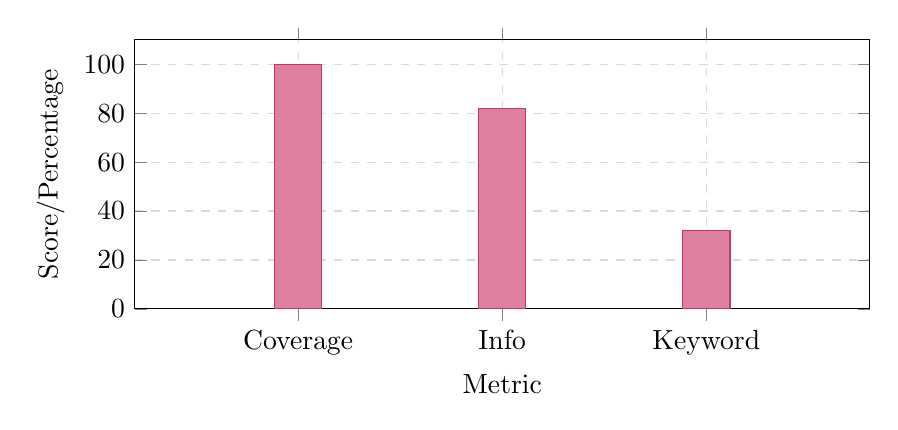
\begin{tikzpicture}
\begin{axis}[
    ybar,
    bar width=0.6cm,
    width=0.9\columnwidth,
    height=5cm,
    ylabel={Score/Percentage},
    xlabel={Metric},
    ymin=0,
    ymax=110,
    xtick=data,
    xticklabels={Coverage, Info, Keyword},
    ytick={0,20,40,60,80,100},
    grid=major,
    grid style={dashed,gray!30},
    enlarge x limits=0.4
]
\addplot[fill=purple!50, draw=purple!80] coordinates {
    (0, 100)
    (1, 82)
    (2, 32)
};
\end{axis}
\end{tikzpicture}
\caption{The Summarization on the other hand shows 100\% coverage, 82 informativeness and a 32\% keywords.}
\label{fig:summarization}
\end{figure}

Figure~\ref{fig:summarization} provides a visual comparison of summarization quality dimensions. The contrast between 100\% coverage and 32\% keyword usage reveals a key advantage of LLM-based summarization: the ability to synthesize information using contextual language rather than merely echoing log keywords. This semantic interpretation capability differentiates our approach from traditional template-based or regex-driven log analysis tools, producing human-readable, actionable output that bridges the gap between machine-generated logs and human operational decision-making.


\section{Future Work}
The future research needs to have a shared and unified benchmark that calculates the anomaly detection, summary accuracy and safety of the system while the testing of the anomaly detection and the AI frameworks will have to be tested all at once to reflect as a one single system. As of the latency budget, it is critical to create a retrieval streaming and summarization that can work under only a strict time limit with the help of concepts as ``Attention-sink'' and ``Chunked processing'' to reduce the amount of tokens used and make our system efficient.


\section{Conclusion}
We created a strong way to reform the messy systems into helpful ones by combining the LLMs with the MCP, focusing on real world systems that are practical for various data log sources. With the help of AI any kind of logs can be cleared and shortened, and when the AI needs to run a command it does it through a secure protocol that tracks everything, making the system safe and auditable. All the data the system outputs from logs to incident history is securely saved.
\section*{Acknowledgment}

\begin{enumerate}
  \item \textbf{The Funding:} There is no applicable funding.
  \item \textbf{Conflicts of interest:} There is no conflict of interest.
  \item \textbf{Ethics approval and consent:} There is no applicable approvals.
  \item \textbf{Consent for publication:} All authors have provided the consent needed for our research.
  \item \textbf{Data availability:} All data used here is publicly available as indicated in the relevant sections.
  \item \textbf{Code availability:} \url{https://github.com/zakzakkhkh/llm-log-responder}
\end{enumerate}

\begin{thebibliography}{99}

\bibitem{du2017deeplog}
M. Du, F. Li, G. Zheng, and V. Srikumar, ``DeepLog: Anomaly detection and diagnosis from system logs through deep learning,'' in \textit{Proc. ACM SIGSAC Conf. Comput. Commun. Security (CCS)}, Dallas, TX, USA, 2017, pp. 1285--1298.

\bibitem{meng2019loganomaly}
W. Meng, Y. Lin, J. Liu, S. Zhang, M. Zhang, J. Li, M. R. Lyu, and I. King, ``LogAnomaly: Unsupervised detection of sequential and quantitative anomalies in unstructured logs,'' in \textit{Proc. 28th Int. Joint Conf. Artif. Intell. (IJCAI)}, Macao, China, 2019, pp. 4739--4745.

\bibitem{guo2021logbert}
H. Guo, L. Zhang, J. Wang, L. Nie, X. Luo, and X. Qian, ``LogBERT: Log anomaly detection via BERT,'' in \textit{Proc. IEEE Int. Conf. Softw. Anal., Evol. Reeng. (SANER)}, Honolulu, HI, USA, 2021, pp. 1--8.

\bibitem{liu2023geval}
Y. Liu, A. Nie, A. Chaganty, et al., ``G-Eval: NLG evaluation using GPT-4 with better human alignment,'' arXiv preprint arXiv:2303.16634, 2023.

\bibitem{xiao2023streamingllm}
G.-X. Xiao, H. Dong, Y. Yu, et al., ``Efficient streaming language models with attention sinks,'' arXiv preprint arXiv:2309.17453, 2023.

\bibitem{zou2023universal}
A. Zou, Z. Wang, A. D'Amour, et al., ``Universal and transferable adversarial attacks on aligned language models,'' arXiv preprint arXiv:2307.15043, 2023.

\bibitem{zhang2019bertscore}
T. Zhang, V. Kishore, F. Wu, K. Q. Weinberger, and Y. Artzi, ``BERTScore: Evaluating text generation with BERT,'' in \textit{Proc. Int. Conf. Learn. Represent. (ICLR)}, New Orleans, LA, USA, 2020.

\bibitem{manakul2023selfcheck}
P. Manakul, A. Liusie, and M. J. F. Gales, ``SelfCheckGPT: Zero-resource black-box hallucination detection for generative large language models,'' in \textit{Proc. Conf. Empirical Methods Natural Lang. Process. (EMNLP)}, Singapore, 2023, pp. 9004--9017.

\bibitem{zhang2024promptinj}
N. Zhang, J. Chen, B. Li, et al., ``Prompt injection attacks and defenses in LLM-integrated applications,'' arXiv preprint arXiv:2310.12815, 2024.

\bibitem{yao2022react}
S. Yao, D. Yu, J. Zhao, I. Shafran, T. L. Griffiths, Y. Cao, and K. Narasimhan, ``ReAct: Synergizing reasoning and acting in language models,'' in \textit{Proc. Int. Conf. Learn. Represent. (ICLR)}, Kigali, Rwanda, 2023.

\bibitem{schick2023toolformer}
T. Schick, J. Dwivedi-Yu, R. Raileanu, et al., ``Toolformer: Language models can teach themselves to use tools,'' in \textit{Proc. Conf. Neural Inf. Process. Syst. (NeurIPS)}, New Orleans, LA, USA, 2023, pp. 10087--10101.

\bibitem{wu2023autogen}
T. Wu, B. Zhang, Z. Xu, et al., ``AutoGen: Enabling next-gen LLM applications via multi-agent conversation,'' arXiv preprint arXiv:2308.08155, 2023.

\bibitem{he2018drain}
P. He, J. Zhu, Z. Zheng, and M. R. Lyu, ``Drain: An online log parsing approach with fixed depth tree,'' in \textit{Proc. IEEE Int. Conf. Web Services (ICWS)}, San Francisco, CA, USA, 2017, pp. 33--40.

\bibitem{reimers2019sbert}
N. Reimers and I. Gurevych, ``Sentence-BERT: Sentence embeddings using siamese BERT-networks,'' in \textit{Proc. Conf. Empirical Methods Natural Lang. Process. (EMNLP)}, Hong Kong, China, 2019, pp. 3982--3992.

\bibitem{owasp2025top10}
OWASP Foundation, ``OWASP Top 10 for large language model applications,'' 2025. [Online]. Available: https://genai.owasp.org/llm-top-10/

\bibitem{mcp}
Anthropic, ``Model Context Protocol (MCP) specification,'' 2024. [Online]. Available: https://modelcontextprotocol.io/

\end{thebibliography}

\end{document}


